% !TeX root = ../../Thesis.tex
\chapter{Effects of an External Magnetic Field on Stimulated Raman Scattering in homogeneous plasmas}
\label{chp:magSRS}

In this chapter, we present work performed while on a research placement at the University of California, San Diego between January and May 2020. The final few weeks of the project were interrupted by Covid-19, and were completed remotely from my parents' home. The work presented (including data generated and data analysis) was carried out by the author, except in the cases outline below:
\begin{itemize}
\item Figure \ref{fig:SRS_LULI} SRS reflectivity from LULI, made by Matthieu
\end{itemize}

The chapter begins with a review of the literature which discusses the effect of an externally-applied magnetic field on stimulated Raman scattering. We then present modelling performed by the author of an experiment performed on the LULI laser system in France by: LIST OF EXPERIMENTALISTS, with analysis of the diagnostics performed by: Adam Higginson; Matthieu Bailey Grandeaux. The experiment showed a small increase in SRS with an applied magnetic field, and this is recreated in our simulations. We then go on to investigate how the effect of the magnetic field depends on $\kld$ of the SRS electron plasma wave.

\section{Motivation and literature review}

here's a recent paper about 90T fields effect on SRS in inhomogeneous plasmas \citep{Zhou2021}. 

Start by replicating results from \cite{Winjum2018}

Suppress SRS to reduce harmful electrons and reflectivity, or enhance if it actually makes good electrons (in the case of shock-ignition)

\section{Modelling SRS on LULI}
\subsection{Experimental results}
\begin{figure}[ht]
   \centering
    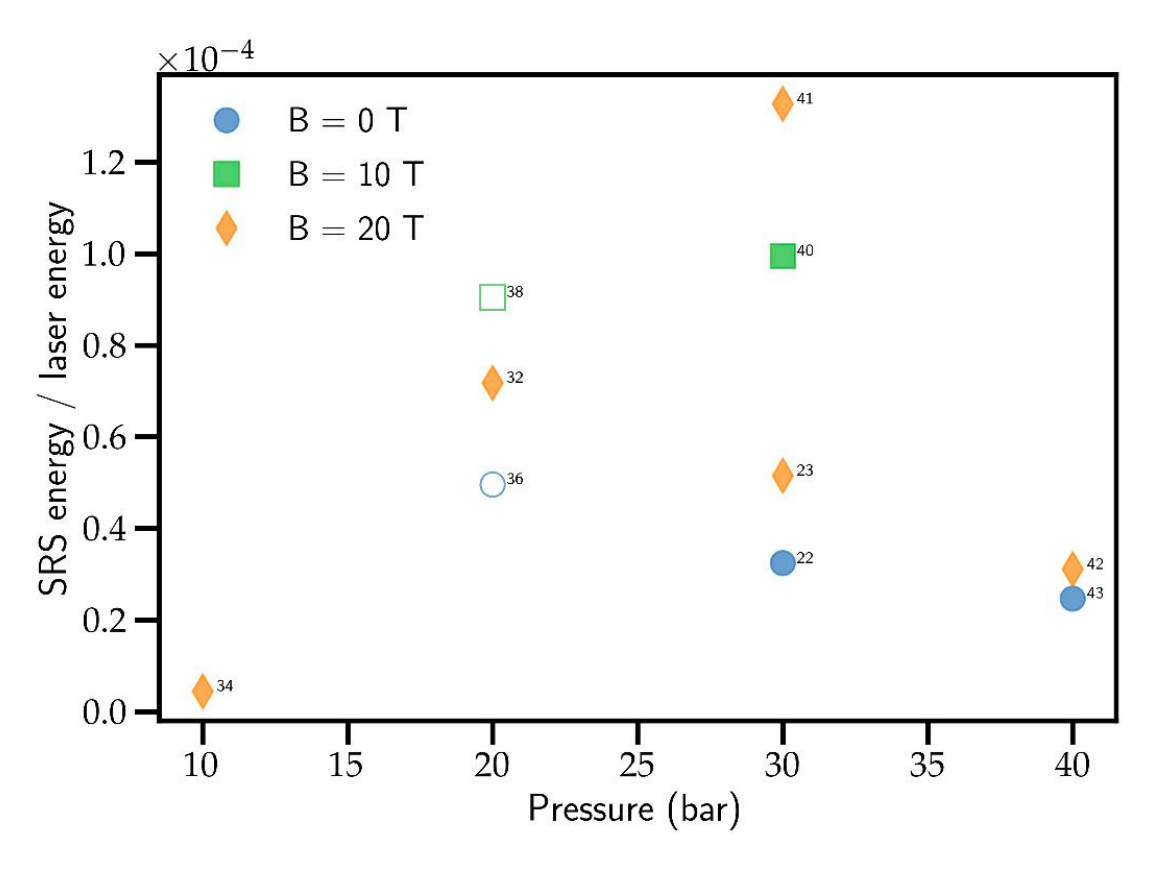
\includegraphics[width=0.75\columnwidth]{Chapters/C6_magSRS/SRS_LULI.png}
    \caption{MAthieu made this}
    \label{fig:SRS_LULI}
\end{figure}{}


\subsection{Simulation results}

\section{Magnetic field effect varies with plasma debye length}
\subsection{Rescatter}
\subsection{Kinetic inflation}
\subsection{Trapped particle modulation instability}
\subsection{Langmuir decay instability}

\section{Magnetic field effect changes with polarisation}




